\chapter{Diseño e implementación} % Main chapter title

\label{Chapter3} % Change X to a consecutive number; for referencing this chapter elsewhere, use \ref{ChapterX}

En este capítulo se explica como se diseño el dispositivo, como esta conformado el hardware y software del equipo y como se desarrolló la aplicación para control del motorhome. 


\section{Desarrollo de hardware}
\label{sec:desarrollo_hardware}

A continuación, se explicarán como se desarrollaron los distintos módulos de hardware del equipo y como se relacionan unos con otros. Como se mencionó anteriormente, el ESP32 debe actuar como intermediario y vínculo entre las tres partes principales: módulo PRC10, Cerbo GX y aplicación móvil.

La figura \ref{fig:esquema_hw_general} muestra una estructura del flujo o camino que debe seguir el ESP32 para llegar a cada una de estas partes.


\begin{figure}[h]
	\centering
	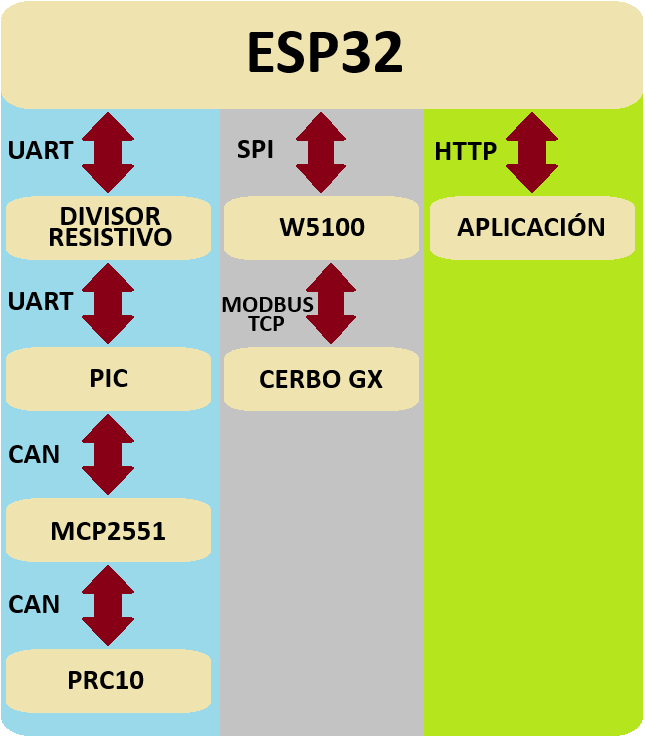
\includegraphics[scale=0.55]{./Figures/esquema_hw_general.png}
	\caption{Trayecto que sigue el ESP32 para llegar a cada uno de los módulos.}
	\label{fig:esquema_hw_general}
\end{figure}

La columna celeste representa la forma de comunicar el ESP32 con el módulo PRC10. Asimismo, las columnas gris y verde representan los caminos hacia el Cerbo GX y aplicación móvil respectivamente.


\subsection{Comunicación con la red Enertik}

Como se mencionó en la sección \ref{sec:protocolo_can}, la red de
domótica de Enertik utiliza una biblioteca propia basada en el
protocolo CAN. A su vez, todos los dispositivos de la red se conectan
a través de un cableado de cuatro conductores: dos destinados a la
alimentación de los equipos y dos destinados a la comunicación CAN
(CAN H y CAN L).

Para el desarrollo de la comunicación del ESP32 mediante este
protocolo, se consideró en primer lugar la adaptación de la biblioteca
de Enertik dentro del firmware del dispositivo. Durante la etapa de
investigación se identificaron bibliotecas disponibles que permiten al
ESP32 implementar comunicación CAN a través de sus puertos GPIO.

Sin embargo, los intentos de establecer una comunicación básica entre
el ESP32 y el módulo PRC10 no arrojaron resultados satisfactorios.
Esto se debe a la complejidad de la biblioteca propia desarrollada por
Enertik, cuyas condiciones y configuraciones no pudieron ser
replicadas en el ESP32.

Ante esta situación, se analizaron alternativas disponibles dentro de
los equipos comercializados por Enertik. En este contexto, se identificó
un módulo transceiver (mostrado en la figura \ref{fig:im_hw_transceiver}) utilizado en conjunto con la pantalla HMI de control. Esta placa tiene como función realizar la conversión del
protocolo CAN, proveniente de la red del motorhome, a una interfaz de
comunicación UART, compatible con la pantalla.

\begin{figure}[h]
	\centering
	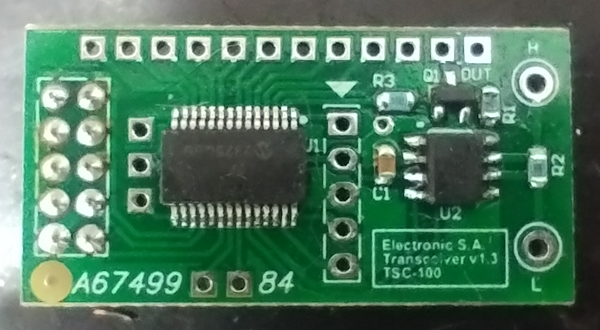
\includegraphics[scale=0.6]{./Figures/placa_transceiver.png}
	\caption{Módulo transceiver comercial perteneciente a Enertik.}
	\label{fig:divisor_resistivo}
\end{figure}

Basado en esta premisa, se decidió replicar y adaptar este módulo transceiver
para que sea compatible con el dispositivo basado en ESP32. Este
módulo se compone de un microcontrolador PIC y de un transceptor CAN
MCP2551.

La figura \ref{fig:im_hw_transceiver} muestra un diagrama completo sobre como fue la implementación de este módulo transceiver.

\begin{figure}[h]
	\centering
	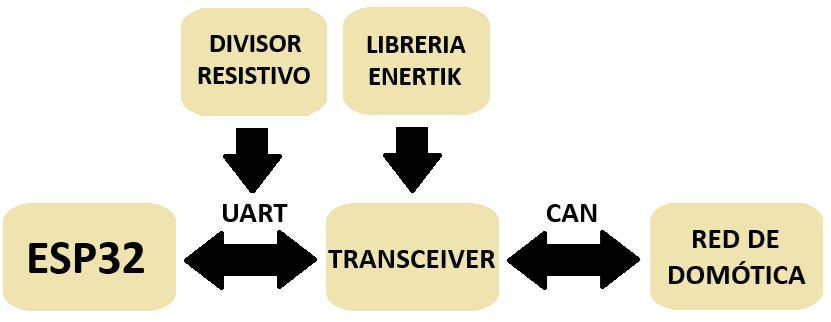
\includegraphics[scale=0.6]{./Figures/esquema_hw_transceiver.png}
	\caption{Diagrama de como se estable la comunicación CAN entre la red del motorhome y el ESP32.}
	\label{fig:im_hw_transceiver}
\end{figure}
\newpage
El microcontrolador PIC dispone de la biblioteca de comunicación
propia desarrollada por Enertik, lo que le permite interactuar de forma
nativa con la red de domótica del motorhome. Por su parte, el
transceptor MCP2551 se encarga de la adaptación de niveles eléctricos
necesarios para la transmisión diferencial sobre el bus CAN.

El microcontrolador PIC funciona con una tensión de alimentación de
5 V, mientras que el ESP32 opera con 3,3 V. Esto implica que los niveles
de tensión utilizados en los puertos UART de cada dispositivo son
diferentes.

Esta diferencia generó la necesidad de adaptar los niveles de tensión
en la comunicación UART, ya que una conexión directa podría dañar los
puertos del ESP32 debido a su menor tolerancia de voltaje.

La solución adoptada fue la implementación de un divisor resistivo. La
figura \ref{fig:divisor_resistivo} muestra un diagrama del circuito
utilizado, junto con el cálculo correspondiente a la tensión de salida.

\begin{figure}[h]
	\centering
	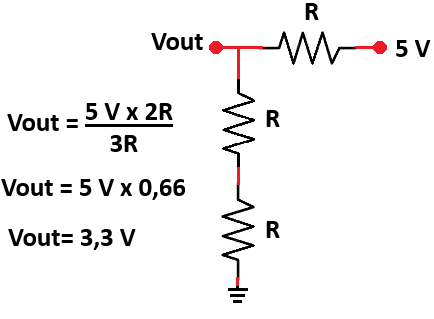
\includegraphics[scale=0.6]{./Figures/divisor_resistivo.png}
	\caption{Diseño de divisor resistivo para adaptación UART.}
	\label{fig:divisor_resistivo}
\end{figure}

Mediante el uso de tres resistencias de igual valor, se logró reducir la
tensión de 5 V a 3,3 V en la línea de transmisión hacia el ESP32,
lo que permitió una comunicación segura entre ambos dispositivos.
\newpage
Este divisor fue implementado en la conexión correspondiente a la línea
de transmisión UART (Tx) del microcontrolador PIC hacia la línea de
recepción UART (Rx) del ESP32. En el sentido contrario no fue necesaria
esta adaptación, ya que el nivel lógico de 3,3 V proveniente del ESP32
es reconocido correctamente por el PIC.

De esta manera, el módulo transceiver actúa como un intermediario que
realiza la conversión entre la red CAN y una interfaz UART. Esto
permite que el ESP32 pueda enviar y recibir información de la red de
domótica sin necesidad de implementar directamente la complejidad del
protocolo CAN utilizado por Enertik.


\subsection{Comunicación con la red Victron}

La comunicación con la red Victron se realizó mediante el protocolo
Modbus TCP. Desde el punto de vista del hardware, el microcontrolador
ESP32 no dispone de una interfaz Ethernet integrada, por lo que fue
necesario incorporar un módulo externo que permita este tipo de
conectividad.

Durante la etapa de investigación se analizaron distintas alternativas
para implementar la comunicación Ethernet. Como resultado, se optó por
utilizar el módulo W5100, debido a su amplia disponibilidad en el
mercado, su bajo costo y su compatibilidad con entornos de desarrollo
basados en Arduino.

Adicionalmente, el IDE Arduino dispone de bibliotecas específicas para
la comunicación Ethernet que resultan compatibles con este módulo, lo
que facilitó su integración dentro del sistema. Estas características
hicieron del W5100 una opción adecuada para la implementación de la
comunicación Modbus TCP con los equipos del ecosistema Victron.

Otra ventaja de este componente es que utiliza el protocolo de
comunicación SPI. El ESP32 dispone de periféricos compatibles con este
protocolo, lo que facilitó su integración dentro del sistema.

Más allá del conexionado SPI (pines MOSI, MISO, SCK y CS), la conexión
entre el ESP32 y el W5100 no requirió hardware adicional.

Este módulo funciona con una tensión de alimentación de 5 V, lo que lo
vuelve compatible con el diseño implementado, ya que se aprovecha la
misma fuente utilizada para energizar el microcontrolador PIC del
módulo transceiver.

La conexión Ethernet que parte desde el módulo W5100 se realiza a
través de un conector RJ45. Este conector permite la utilización de
cables de red estándar, compuestos por pares trenzados de conductores,
diseñados para la transmisión de datos a alta velocidad.

Estos cables emplean una transmisión diferencial sobre cada par, lo que
reduce la susceptibilidad a interferencias electromagnéticas y mejora
la integridad de la señal. De esta manera, se garantiza una comunicación
confiable entre el dispositivo desarrollado y la red del sistema
Victron.

Mediante este tipo de conexión, el módulo W5100 puede integrarse
directamente a la red Ethernet donde se encuentra el módulo Cerbo GX,
permitiendo el intercambio de datos necesario para la implementación
del protocolo Modbus TCP.

Para lograr la comunicación, resta definir qué dispositivo cumplirá el
rol de maestro y cuál el de esclavo. Esta definición se abordará en la
sección de firmware, donde se detallará su implementación.

\subsection{Prototipo experimental}

Para realizar los primeros ensayos, se decidió montar un primer
prototipo del equipo. Para ello, se utilizó como base un PCB perforado
de tipo experimental, sobre el que se soldaron diversos conectores,
cableados y componentes de forma manual.

La figura \ref{fig:prototipo_experimental} muestra el resultado del
montaje del prototipo utilizado para los ensayos iniciales.

\begin{figure}[h]
	\centering
	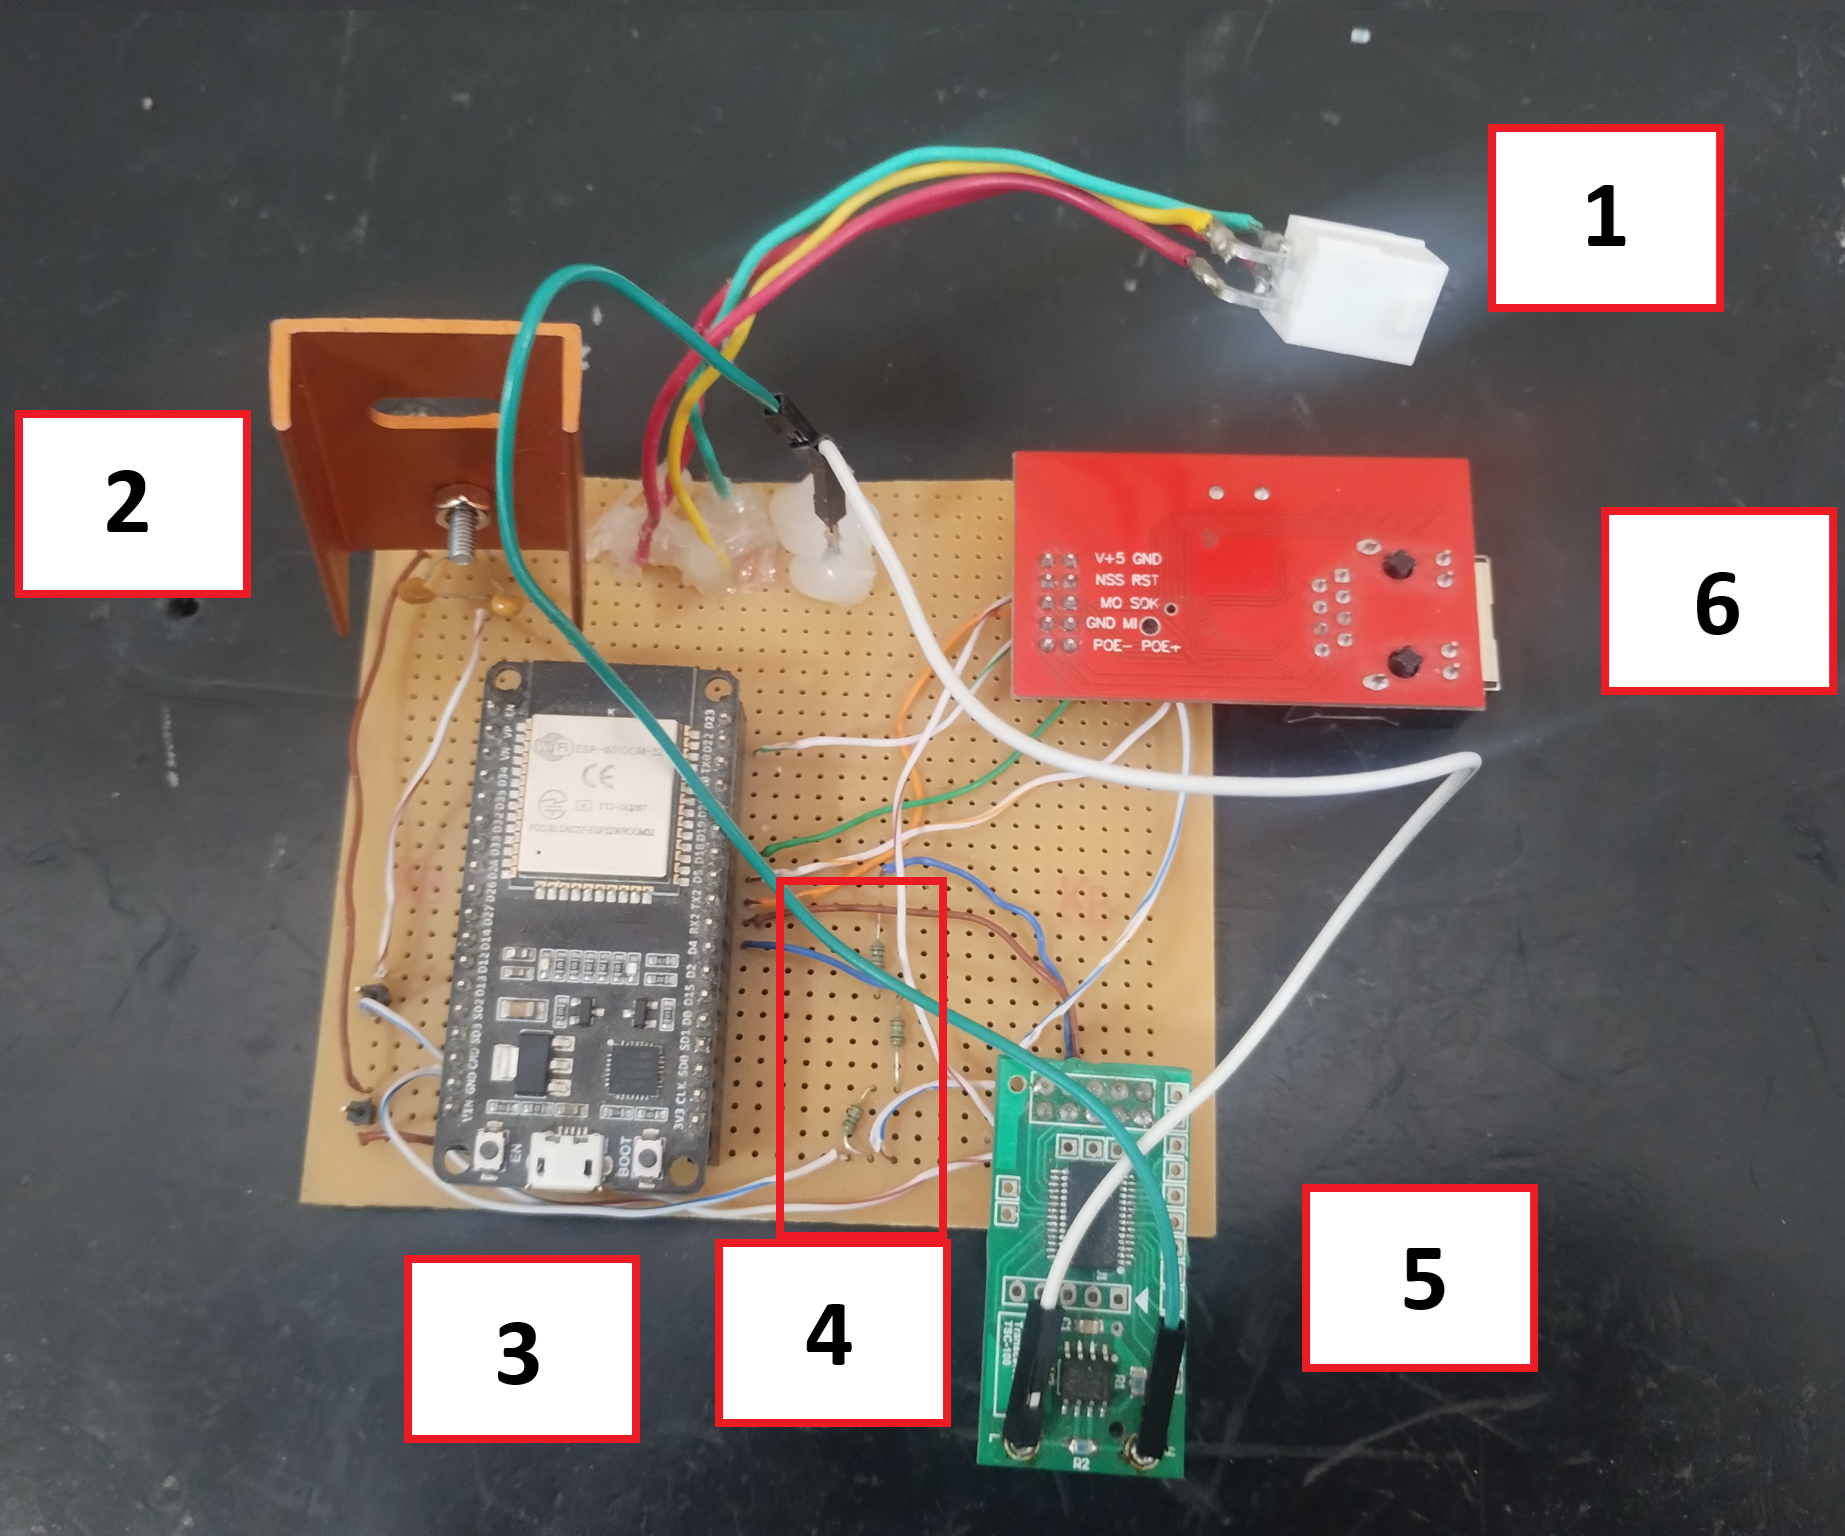
\includegraphics[scale=0.27]{./Figures/prototipo_experimental.png}
	\caption{Prototipo experimental del equipo.}
	\label{fig:prototipo_experimental}
\end{figure}

Como se puede apreciar, el prototipo cuenta con cada uno de los módulos
explicados en secciones anteriores, donde:

\begin{itemize}
    \item Componente 1: conector de cuatro hilos. Este conector es el estándar empleado en la red de domótica de Enertik. A través de él se energizan todos los componentes del PCB experimental y se accede a la comunicación CAN de la red.
    
    \item Componente 2: regulador de tensión 7805 \citep{7805_datasheet}. Este dispositivo se encarga de suministrar una tensión estable de 5 V. Dado que la tensión proveniente del motorhome es de 12 V, fue necesaria su utilización para adecuar los niveles de alimentación a los requeridos por los módulos.
    
    \item Componente 3: módulo ESP32. Es el microcontrolador principal de la placa y contiene el firmware de control del sistema. En este prototipo se alimentó a través del regulador 7805, ya que la placa de desarrollo dispone internamente de reguladores que reducen la tensión a 3,3 V. Para el desarrollo final fue necesaria la incorporación de un regulador adicional dedicado al ESP32.
    
    \item Componente 4: divisor resistivo. Corresponde al arreglo de resistencias encargado de adaptar los niveles de tensión y permitir una comunicación UART segura entre el ESP32 y el módulo transceiver.
    
    \item Componente 5: módulo transceiver. Se trata de una placa comercial provista por Enertik. En este prototipo se decidió incorporar un conector en el PCB experimental para facilitar su montaje y desmontaje de forma segura.
    
    \item Componente 6: módulo W5100. De manera similar al módulo transceiver, se utilizó un conector compatible que permite su montaje y desmontaje de forma sencilla y segura.
\end{itemize}

Este prototipo permitió validar el funcionamiento general del sistema
y realizar pruebas iniciales de integración entre los distintos módulos
de hardware.

\subsection{Desarrollo de PCB final y listado de componentes}

El diseño del PCB final se desarrolló mediante el software Altium
Designer \citep{web_altium}. Este software es ampliamente utilizado en la industria, ya
que permite crear esquemáticos de circuitos de forma sencilla. Estos
esquemáticos sirven como base para el diseño de placas de circuito
impreso.

Para la creación de este PCB, se tomó como referencia el conexionado
utilizado en el prototipo experimental.

Dado que se espera que este desarrollo se convierta en un producto
comercial, fue necesario realizar modificaciones en la selección de
componentes durante el diseño de este prototipo.

La primera diferencia se encuentra en el microcontrolador ESP32. Para
el prototipo experimental y los ensayos iniciales se utilizó una placa
de desarrollo comercial basada en este dispositivo.

En el diseño del PCB final, se optó por reemplazar dicha placa por el
chip del microcontrolador en sí. Esta decisión permitió descartar los
componentes adicionales presentes en la placa de desarrollo. De esta
forma, se eliminó hardware innecesario, se redujeron costos y se
optimizó el espacio disponible en el PCB.

Por otra parte, fue necesaria la incorporación de un regulador de
tensión AP63203 \citep{AP63203_datasheet}. Este dispositivo permite adaptar el nivel de tensión
de 12 V proveniente de la red del motorhome a un valor de 3,3 V,
compatible con el chip ESP32.

En el caso del módulo transceiver, dado que se conocía completamente su
diseño, se optó por integrarlo directamente en el PCB. Para ello, se
incorporaron el microcontrolador PIC18F26K60 y el transceptor MCP2551
en la placa. Esta decisión permitió optimizar el espacio disponible y
reducir costos al unificar todos los componentes en una única placa.

En cuanto al módulo W5100, se optó por utilizar la versión comercial
disponible en el mercado. Inicialmente se evaluó realizar un proceso de
ingeniería inversa para analizar su diseño interno, pero se descartó
esta alternativa debido al tiempo requerido.

Como consecuencia, en el PCB se reservó un espacio para la colocación
de un conector compatible con el módulo W5100, lo que permite su
montaje manual de forma sencilla.

En la figura \ref{fig:pcb_final} se puede observar el diseño final del PCB.

\begin{figure}[h]
	\centering
	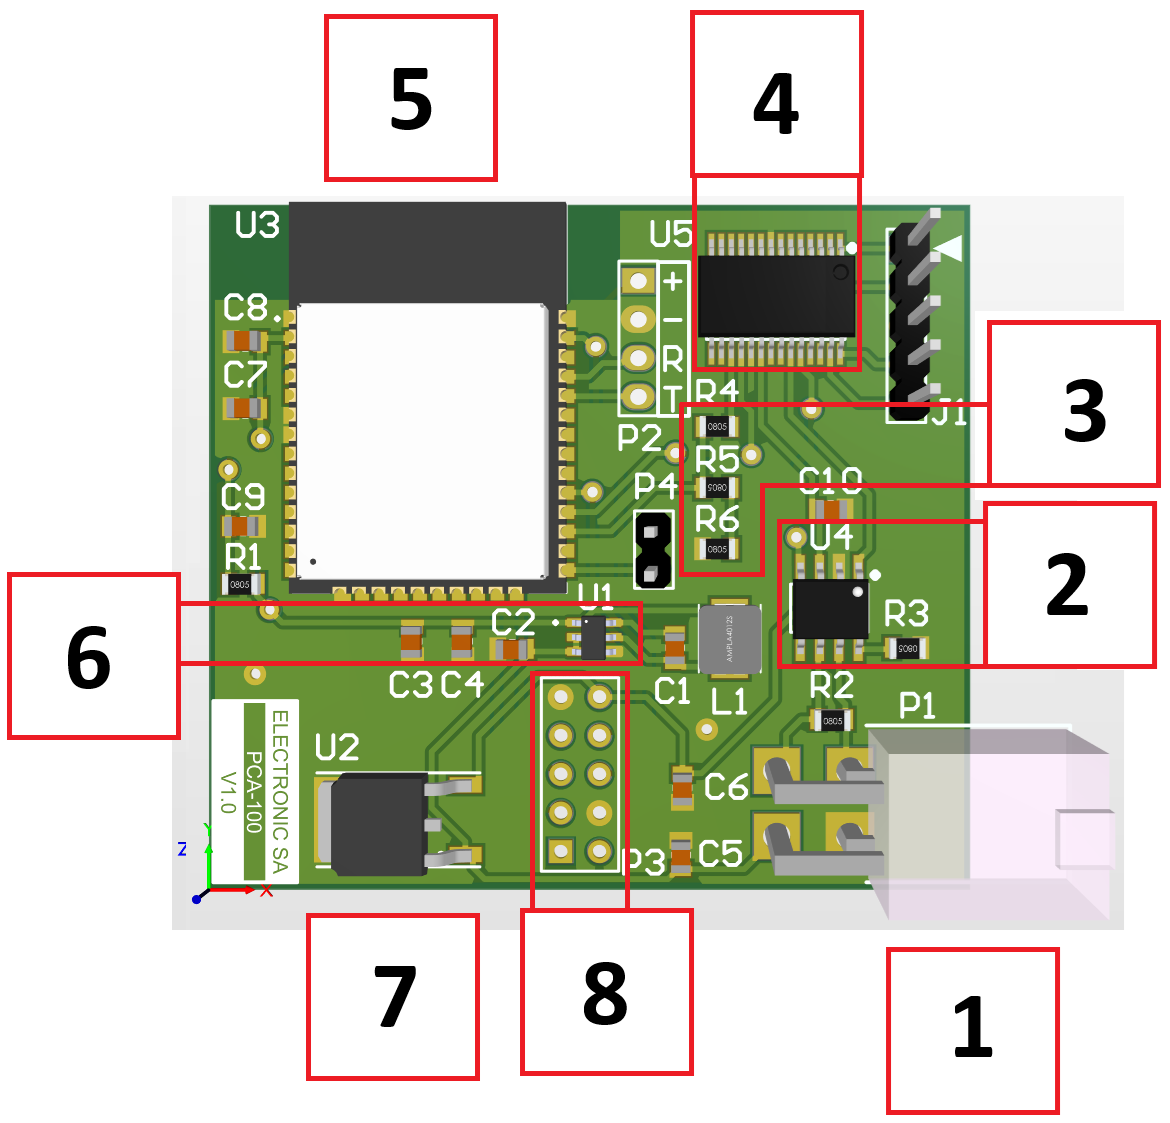
\includegraphics[scale=0.4]{./Figures/pcb_pca10.png}
	\caption{Diseño final para PCB del equipo.}
	\label{fig:pcb_final}
\end{figure}

Como se puede apreciar, el PCB esta compuesto por los siguientes componentes:

\begin{itemize}
	\item Componente 1: conector principal. Terminal sobre que se conecta el cableado de cuatro hilos proveniente del motorhome.
	\item Componente 2: MCP2551. Forma parte del módulo transceiver, encargado de adaptar los niveles de tensión de la linea CAN.
	\item Componente 3: divisor resistivo. Corresponde al arreglo de resistencias encargado de adaptar los niveles de tensión y permitir una comunicación UART segura entre el ESP32 y el módulo transceiver.
	\item Componente 4: PIC18F26K80. Microcontrolador que contiene la biblioteca desarrollada por Enertik para la comunicación entre equipos.
	\item Componente 5: módulo ESP32. Microcontrolador que contiene el firmware principal del equipo.    
    \item Componente 6: regulador de tensión AP63203. Fuente de tensión de 3,3 V encargado alimentar el ESP32.
    \item Componente 7: regulador de tensión 7805. Componente responsable de suministrar una tensión estable de 5 V para alimentar el PIC y el W5100.   
    \item Componente 8: conector de diez pines. Conector compatible con el módulo W5100. En este lugar se montará dicho componente.
\end{itemize}

Para el proceso de fabricación, fue necesaria la contratación de
servicios de un fabricante especializado en este campo. Para ello, se
generaron los denominados archivos Gerber \citep{web_altiu_gerber}.

Los archivos Gerber constituyen el estándar utilizado en la industria
para describir las distintas capas de una placa de circuito impreso.
Cada archivo representa una capa específica del PCB, como las pistas de
cobre, la máscara de soldadura, la serigrafía o el plano de taladros.
A partir de esta información, el fabricante puede interpretar el diseño
y llevar a cabo la fabricación física de la placa con precisión.

A modo de resumen, se deja una tabla que lista los principales componentes empleados para la fabricación del PCB.

\begin{table}[h]
	\centering
	\caption[Componentes utilizados en el PCB final.]{Componentes utilizados en el PCB final.}
	\begin{tabular}{m{2cm} m{8cm}}   
		\toprule
		\textbf{Componente} 	 & \textbf{Descripción} \\
		\midrule
		ESP32		&	Microcontrolador principal del equipo. \\		
		PIC18F26K80		&	Encargado de la comunicación CAN. \\
		MCP2551		&	Encargado de adaptación de niveles en la comunicación CAN.\\
		7805		&	Regulador de tensión de 5 V.\\
		AP63203		&	Regulador de tensión de 3,3 V.\\
		Resistencias		&	Arreglo para el divisor de tensión.\\
		W5100		&	Módulo para comunicación Ethernet.\\
		\bottomrule
		\hline
	\end{tabular}
	\label{tab:dut}
\end{table}

\section{Desarrollo de firmware}
\label{sec:desarrollo_firmware}

Como se mencionó en la sección \ref{sec:rtos}, se optó por utilizar
FreeRTOS como base para el desarrollo del firmware.

FreeRTOS permite estructurar el firmware mediante la ejecución de
múltiples tareas. La planificación de estas tareas genera un
comportamiento concurrente a nivel lógico, lo que mejora la organización
del sistema y facilita la gestión de sus funcionalidades.

En este contexto, en el presente trabajo se implementaron seis tareas
principales.

\subsection{Tarea: recepción UART}

Esta tarea se encarga de escuchar constantemente el puerto UART del
ESP32. Cada vez que se detecta una señal en sus puertos, la tarea
almacena la información recibida en un buffer de tipo circular \citep{ringbuffer}.

Un buffer circular, también conocido como \textit{ring buffer}, es una
estructura de datos que utiliza una región de memoria de tamaño fijo y
organiza los datos de forma continua. Cuando se alcanza el final del
buffer, la escritura continúa desde el inicio, lo que permite reutilizar
la memoria de manera eficiente sin necesidad de realizar desplazamientos
de datos.

Se opt[o por este tipo de estructura porque resulta especialmente adecuado para la recepción
de datos en tiempo real, ya que permite desacoplar la velocidad de llegada
de la información respecto de su procesamiento. De esta forma, se evita la
pérdida de datos ante ráfagas de información y se garantiza un manejo más
robusto de la comunicación UART.


\subsection{Tarea: decodificación de comando CAN}
\label{sec:comando_can}
Esta tarea se encarga de decodificar los comandos recibidos desde la
red CAN. Para ello, realiza la lectura de los datos almacenados en el
buffer circular.

La información transmitida en la red CAN sigue un formato
predefinido. El primer byte corresponde a una marca de inicio, que
permite identificar el comienzo de cada trama. Por otro lado, el último
byte corresponde a un valor de control CRC (\textit{Cyclic Redundancy Check}),
utilizado para verificar la integridad de los datos recibidos mediante
un cálculo basado en el contenido del mensaje.

Dentro de la trama de datos se incluyen los campos de dirección de
origen, que identifica el dispositivo emisor, dirección de destino,
que indica el dispositivo receptor, un campo de comando asociado a la
acción a ejecutar y un conjunto de bytes de datos.

Esta tarea se encarga de analizar cada trama completa. Para ello, recorre el buffer
circular hasta encontrar el byte de marca de inicio.

A continuación, extrae la trama completa y realiza el cálculo del CRC,
lo que permite determinar si la trama es válida o no. En caso afirmativo, se
procede a identificar los campos que componen el mensaje.

Cuando se detecta una trama válida, la información útil se transfiere a
la siguiente tarea, encargada de procesar la instrucción correspondiente.


\subsection{Tarea: comunicación Modbus TCP}
\label{sec:comando_modbus}
Esta tarea se encarga de gestionar de manera completa la comunicación
Modbus TCP y, por lo tanto, es responsable del control del módulo
Cerbo GX.

Para establecer la comunicación mediante este protocolo, fue necesario
realizar una serie de configuraciones iniciales.

Se definió que el ESP32 ejerza el rol de maestro, encargado de
solicitar datos y enviar comandos al Cerbo GX.

La comunicación entre ambos dispositivos se realiza a través de un
cable Ethernet con conector RJ45, que vincula el Cerbo GX con el
módulo W5100 controlado por el ESP32.

Para que esta comunicación sea posible, fue necesario definir
direcciones IP estáticas para ambos dispositivos. Esto permite que cada
equipo conozca la dirección del otro y mantenga una comunicación
consistente en el tiempo. Además, ambos deben pertenecer a la misma red,
lo que implica compartir la misma máscara de subred y una configuración
de puerta de enlace (gateway) compatible.

La dirección IP del Cerbo GX se configura desde el menú del propio
equipo. Por otro lado, la dirección IP del ESP32 se definió por
software dentro de esta tarea.

Esta tarea utiliza un contador interno que cumple la función de
temporizador. En primer lugar, establece la comunicación Modbus TCP y
la mantiene activa durante el funcionamiento del sistema.

Posteriormente, en intervalos periódicos, realiza la lectura de los
registros que el Cerbo GX pone a disposición para la obtención de datos
y el control del comportamiento del equipo.

El equipo utilizado para los ensayos fue un Victron Multiplus II
48/5000/70-50, provisto por la empresa Enertik. Si bien el desarrollo
del firmware se realizó sobre este modelo, los registros utilizados
resultan compatibles con otros equipos de la misma línea de
inversores/cargadores Victron.

En este contexto, los parámetros de interés fueron aquellos asociados
al modo de operación del equipo, ya sea en modo inversor o cargador.

Victron dispone de un registro que adopta distintos valores según el
estado del equipo: modo inversor, modo cargador, funcionamiento
combinado o estado apagado. A partir de la lectura de este registro es
posible determinar el estado del equipo en todo momento.

Además, este registro admite operaciones de lectura y escritura, lo que
permite modificar el comportamiento del equipo mediante la asignación
de valores adecuados.

Otros parámetros relevantes incluyen la potencia suministrada por el
equipo en modo inversor y la corriente de carga de entrada en modo
cargador.

\subsection{Tarea: pedido de datos}
\label{sec:pedido_datos}
Esta tarea se encarga de solicitar de forma periódica información al
módulo PRC10.

Dentro de la red de Enertik, el PRC10 actúa como unidad central de
procesamiento. En este módulo se concentran los valores y estados de
todas las variables del motorhome.

Para que la aplicación pueda reflejar esta información en pantalla,
resulta necesario que el ESP32 tenga acceso a dichos datos.

Con este objetivo, fue necesario realizar una modificación en el
firmware del módulo PRC10. Se incorporó una función que permite generar
una serie de paquetes, cada uno asociado a un conjunto de variables del
sistema.

Entre las variables incluidas en estos paquetes se encuentran:

\begin{itemize}
    \item Tensión de batería.
    \item Corriente suministrada por la batería.   
    \item Tensión de entrada en alterna.
    \item Frecuencia de la tensión de entrada.
    \item Origen de la tensión de entrada (red domiciliaria, generador o inversor).
    \item Nivel de llenado de los tanques de agua (limpia, gris y negra).
    \item Estado del cargador.
    \item Corriente de carga.
    \item Estado del inversor.
    \item Potencia suministrada por el inversor.
    \item Estado de los pulsadores asociados a las distintas pantallas de la HMI.
\end{itemize}

Desde el lado del ESP32, esta tarea realiza solicitudes periódicas de
cada uno de estos paquetes. El funcionamiento se basa en un ciclo en el
que, cada 500 ms, se solicita un paquete distinto al PRC10.

Una vez completado el recorrido de todos los paquetes, el proceso se
reinicia desde el primero. Este comportamiento cíclico permite mantener
actualizada la información correspondiente a todas las variables del
sistema.

\subsection{Tarea: procesamiento de comandos recibidos}
\label{sec:procesamiento_comandos}
Esta tarea constituye el núcleo del firmware. Su función principal es
recibir los comandos provenientes de las tareas de comunicación CAN
(\ref{sec:comando_can}) y Modbus TCP (\ref{sec:comando_modbus}), procesarlos
y actualizar las variables internas del sistema.

En relación con la comunicación CAN, esta tarea recibe las tramas ya
validadas por la etapa de decodificación. A partir de estas tramas,
extrae los distintos campos de datos y los interpreta según el tipo de
paquete recibido. Los valores obtenidos se almacenan en estructuras de
datos internas, que representan el estado actualizado de los distintos
sensores y actuadores del motorhome.

Adicionalmente, esta tarea realiza conversiones sobre los datos
recibidos, ya que muchos de ellos se encuentran codificados. Estas conversiones permiten obtener magnitudes físicas en unidades reales, lo que facilita su posterior visualización y
procesamiento.

Por otra parte, la tarea también gestiona comandos destinados al módulo
Cerbo GX a través de Modbus TCP. En función del comando recibido, se
determinan las acciones a ejecutar, como la activación o desactivación
del inversor o del cargador. Para ello, se realiza la escritura sobre
los registros correspondientes del dispositivo Victron, lo que permite
modificar su estado de operación.

Finalmente, una vez procesada la información, los datos actualizados se
envían a otras tareas del sistema a través de colas de FreeRTOS. Este
mecanismo permite desacoplar el procesamiento de datos de su consumo,
mejorando la organización y la escalabilidad del firmware.

\subsection{Tarea: control de servidor}

Esta tarea gestiona la implementación del servidor en el ESP32.

En primer lugar, se encarga de configurar el dispositivo en modo
\textit{Access Point}. En esta modalidad, el microcontrolador genera su
propia red Wi-Fi, lo que permite la conexión directa de otros
dispositivos. Además, se definen los parámetros de la red, tales como
el nombre (SSID) y la contraseña de acceso.

Una vez establecida la conectividad, se definió la estructura del
servidor HTTP mediante la creación de distintos \textit{endpoints}.
Estos representan puntos de acceso que permiten a los clientes
interactuar con el sistema. Cada \textit{endpoint} se asocia a una ruta
específica y a un tipo de solicitud, como GET o POST, lo que permite
consultar información o enviar comandos.

Se optó por implementar un \textit{endpoint} para cada una de las
pantallas principales de la aplicación. Este enfoque permite que cada
pantalla solicite únicamente la información necesaria, lo que reduce el
tráfico de datos y mejora la eficiencia del sistema.

En particular, se definieron cuatro \textit{endpoints} que admiten
solicitudes de tipo GET:

\begin{itemize}
    \item \textit{Home}
    \item Luces  
    \item Motores
    \item Energía
\end{itemize}

Cada uno de estos \textit{endpoints} genera y devuelve un archivo en
formato JSON con la información requerida por la pantalla
correspondiente, lo que permite actualizar la interfaz de usuario con
los valores actuales del sistema.

Por otra parte, la aplicación móvil dispone de distintos pulsadores que
permiten controlar el funcionamiento del motorhome. Para ello, se
implementó un quinto \textit{endpoint} que admite solicitudes de tipo
POST, destinado a la recepción de comandos.

Este \textit{endpoint} recibe un archivo JSON que contiene dos campos:
uno que identifica el pulsador que originó la acción y otro que indica
el nuevo estado asociado.

A partir de esta información, el servidor interpreta el comando y lo
traduce en una instrucción que es enviada al módulo PRC10 para así permitir
la ejecución de la acción correspondiente dentro del sistema.

De esta manera, el servidor implementado en el ESP32 actúa como
intermediario entre la aplicación móvil y la red de domótica,
centralizando tanto la consulta de información como el envío de
comandos.

\section{Desarrollo de la aplicación}
